\subsection{Heap Sort}

\subsubsection{Binary trees}

\begin{minipage}{0.6\textwidth}
    \begin{itemize}
        \item Each node may have a left or a right child (or both)
        \item Each node has at most one parent 
        \item The root has no parent
        \item A leaf has no children
        \end{itemize}
        \end{minipage}
        \begin{minipage}{0.4\textwidth}
            \begin{figure}[H]
                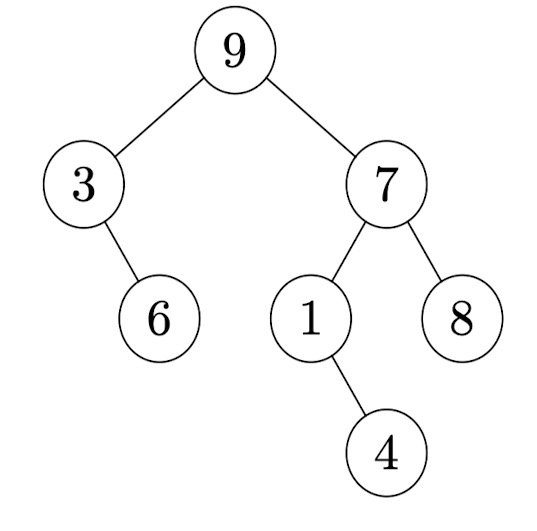
\includegraphics[width=.5\linewidth]{images/Screenshot 2024-05-30 at 14.59.56.jpg}
            \end{figure}
        \end{minipage}
\begin{itemize}
    \item The depth (level) of a node $x$ is the length of the path from the root to $x$
    \item The height of a node $x$ is the length from the longest path from $x$ to a leaf
    \item The height of a tree is the height of its root
    \item The right (left) subtree of a node $x$ is the tree rooted at the right (left) child of $x$
\end{itemize}

\subsubsection{Complete trees}
\begin{itemize}
    \item A \textbf{complete binary tree} is a binary tree where
    \begin{itemize}
        \item all the leaves have the same depth
        \item all internal nodes have two children
    \end{itemize}
        \item A \textbf{nearly complete binary tree} is a binary tree where
        \begin{itemize}
            \item all levels of non-maximal depth $d$ are full (have $2^d$ nodes)
            \item all the leaves with maximal depth are as far left as possible
        \end{itemize}
\end{itemize}

\subsubsection{Heap}
Definition of heap:
\begin{itemize}
    \item A binary tree is a (binary) \textbf{heap} if and only if 
    \begin{itemize}
        \item it is a nearly complete binary tree and, 
        \item each node is greater than or equal to all its children
    \end{itemize}
\end{itemize}
Heaps and arrays are closely related (can use array to represent a heap): 
\begin{figure}[H]
    \centering
    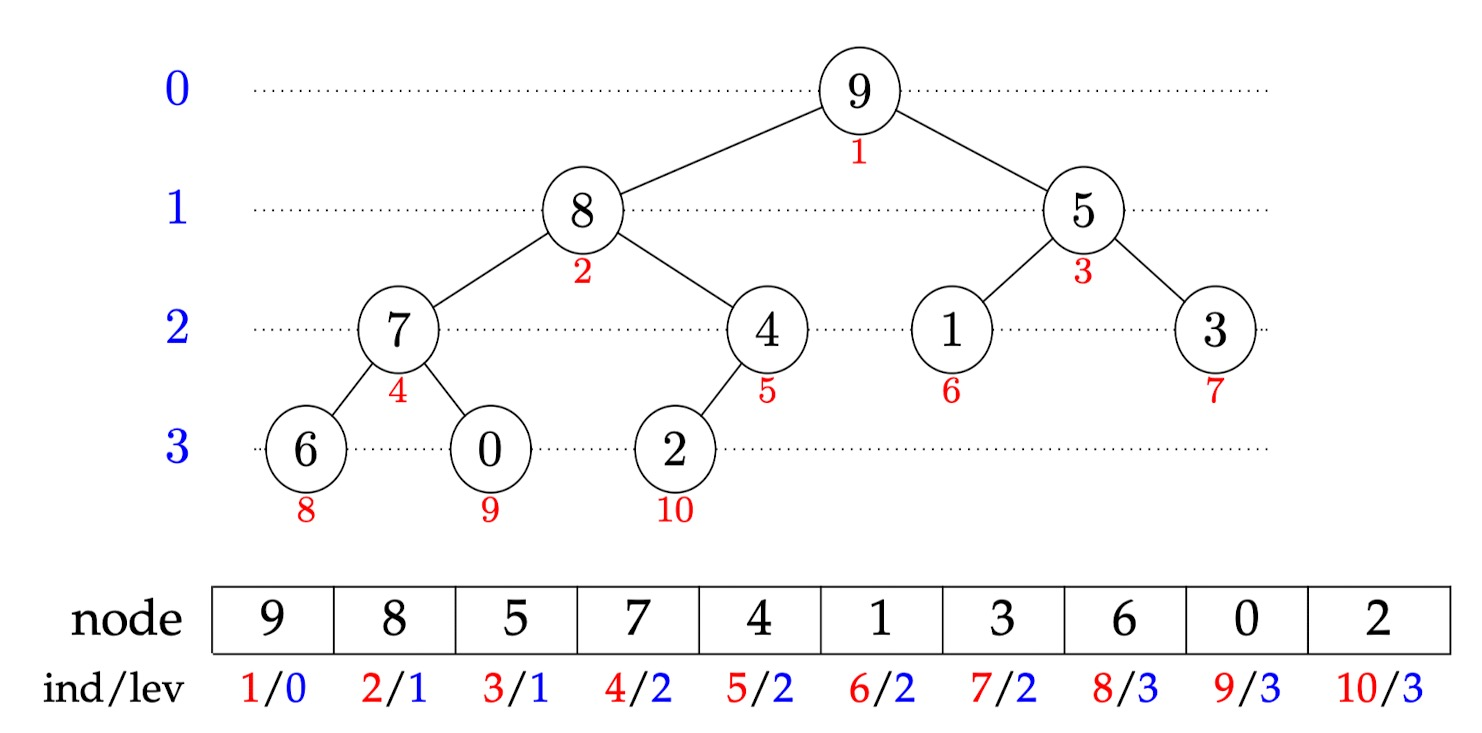
\includegraphics[width=0.75\linewidth]{images/Screenshot 2024-05-30 at 15.11.16.jpg}
\end{figure}

Fundamental properties
\begin{itemize}
    \item Let $i$ be a node index
    \item Heap property: $A[parent(i)]\geq A[i]$
    \item A binary heap can be efficiently stored as an array (because it is a nearly complete binary tree)
    \item Finding parent, left child, and right child:
    \begin{figure}[H]
        \centering
        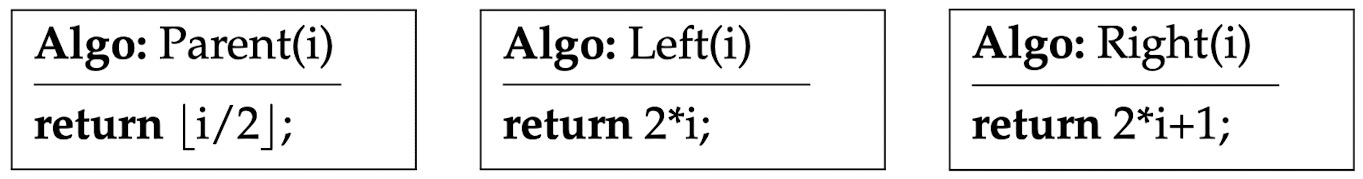
\includegraphics[width=0.5\linewidth]{images/Screenshot 2024-05-30 at 15.13.23.jpg}
    \end{figure}
    \item A heap where the largest (smallest) element is at the root is a max-heap (min-heap)
    \item A binary heap can be exploited for sorting arrays
\end{itemize}

\subsubsection{Heapify}
\begin{itemize}
    \item Input: index $i$ in array $A$, number $s$ of heap elements
    \item Binary trees rooted at \texttt{left}($i$) and \texttt{right}($i$) are binary heaps
    \item $A[i]$ may be smaller than its children, thus violating the heap property
    \item \texttt{heapify}($A,i,s$) transforms the binary tree rooted at $i$ into a binary heap
    \item Strategy: move $A[i]$ down the heap until the heap property is satisfied again
\end{itemize}

\begin{center}
\begin{minipage}{0.6\textwidth} % Adjust the width as needed
\centering % Center the content within the minipage
\begin{algorithm}[H]
\caption{Heapify(A,i,s)}
m = i\;
l = Left(i)\;
r = Right(i)\;
\If{$l<s \land A[l]>A[m]$} {
m = 1\;
}
\If{$r\leq s \land A[r]>A[m]$} {
m = r\;
}
\If{$i\neq m$} {
exchange $A[i]$ and $A[m]$\;
Heapify(A,m,s)\;
}
\end{algorithm}
\end{minipage}
\end{center}

Running time:
\begin{itemize}
    \item The running time of heapify on a subtree of size $n$ rooted at $i$ includes time to 
    \begin{itemize}
        \item determine relationship between elements: $\Theta(1)$
        \item run heapify on a subtree rooted at one of $i$'s children
    \end{itemize}
    \item $2n/3$ is the worst case size of the subtree (half filled bottom level) and thus \[
    T(n) \leq T(2n/3)+\Theta(1), \text{ i.e., } T(n)=O(\log_2 n)
    \]
\end{itemize}

\subsection{Building A Heap}
\begin{itemize}
    \item Convert an array $A$ with $n$ elements into a heap
    \item Note that the elements in $A \left[ \lfloor n/2 + 1 \cdots n \right]$ are 1-element heaps
\end{itemize}

\begin{center}
\begin{minipage}{0.6\textwidth} % Adjust the width as needed
\centering % Center the content within the minipage
\begin{algorithm}[H]
\caption{BuildHeap(A,n)}
\For{$i=\lfloor n/2 \rfloor$ \KwTo 1}{Heapify(A,i,n)\;}
\end{algorithm}
\end{minipage}
\end{center}

Correctness:
\begin{itemize}
    \item Loop invariant: all trees rooted at $m>i$ are heaps
\end{itemize}
Running time:
\begin{itemize}
    \item There are $O(n)$ calls to heapify and so $T(n) = O(n \log_2 n)$
    \item Not an asymptotically tight bound 
    \item Tight bound - Intuition:
    \begin{itemize}
        \item An $n$-element binary heap has height $\log_2 n$
        \item The heap has at most $\lceil[n/2^{h+1}\rceil$ nodes of height $h$
        \item The cost for one call of heapify is $O(h)$
        \item Note: $\sum_{k=0}^\infty kx^k = \frac{x}{(1-x)^2}$
        \item The asymptotically tight bound: 
        \begin{align*}
            T(n) &= \sum_{h=0}^{\log_2 n} \frac{n}{2^{h+1}} O(h) \\
            &= O\left( n\sum_{h=0}^{\log_2 n} \frac{h}{2^{h+1}} \right) \\
            & \leq O\left( n\sum_{h=0}^\infty \frac{h}{2^h}\right)\\
            &= O \left( n\sum_{h=0}^\infty h (1/2)^h\right) \\
            &= O(n\cdot 2) = O(n)
        \end{align*}
    \end{itemize}
\end{itemize}

\subsubsection{Heap Sort Algorithm}

\begin{center}
\begin{minipage}{0.6\textwidth} % Adjust the width as needed
\centering % Center the content within the minipage
\begin{algorithm}[H]
\caption{HeapSort(A,n)}
s = n\;
BuildHeap(A,n)\;
\For{$i=n$ \KwTo 2 }{
exchange A[i] and A[1]\;
s = s-1\;
Heapify(A,1,s)\;
}
\end{algorithm}
\end{minipage}
\end{center}

Running time: 
\begin{itemize}
    \item Heap sort runs in time $O(n)+nO(\log_2 n)=O(n \log_2 n)$
\end{itemize}

\subsection{Quick Sort}
Rough idea:
\begin{itemize}
    \item A divide-and-conquer algorithm
    \begin{itemize}
        \item Divide: partition array into two subarrays such that the items in the lower part $\leq$ the items in the upper part
        \item Conquer: recursively sort the two subarrays
        \item Combine: trivial since sorting is in place
    \end{itemize}
\end{itemize}

\begin{center}
\begin{minipage}{0.6\textwidth} % Adjust the width as needed
\centering % Center the content within the minipage
\begin{algorithm}[H]
\caption{QuickSort(A,l,r)}
\If{$l<r$} {
m = HoarePartition(A,l,r)\;
QuickSort(A,l,m-1)\;
QuickSort(A,m,r)\;
}
\end{algorithm}
\end{minipage}
\end{center}

\begin{center}
\begin{minipage}{0.6\textwidth} % Adjust the width as needed
\centering % Center the content within the minipage
\begin{algorithm}[H]
\caption{HoareParition(A,l,r)}
x = A[r]; i = l-1; j = r+1\;
\While{true} {
\textbf{repeat} j = j-1 \textbf{until} $A[j]\leq x$\;
\textbf{repeat} i = i+1 \textbf{until} $A[i]\geq x$\;
\If{$i<j$}{
exchange A[i] and A[j] \textbf{else return} i\;
}
}
\end{algorithm}
\end{minipage}
\end{center}

\subsubsection{Performance}
Worst case:
\begin{itemize}
    \item Occurs when the array is already completely sorted
    \item Partitioning produces one subproblem with $n-1$ items and one with 1 item
    \item If such a partitioning arises at each recursive call then \[
    T(n)=T(n-1)+T(1) + \Theta(n) =T(n-1)+\Theta(n)
    \] where $\Theta(n)$ is the cost of partitioning the array
    \item Sum of the costs incurred at each level of the recursion yields an arithmetic series (i.e., $\sum_{i=1}^n i = \Theta(n^2)$
\end{itemize}
Best case:
\begin{itemize}
    \item Partitioning produces two subproblems of size $n/2$
    \item If such a partitioning arises at each recursive call then \[
    T(n)=2T(n/2)+\Theta(n)
    \]
    \item It thus follows that, in the best case, $T(n)=\Theta(n \log_2 n)$
\end{itemize}
Average case:
\begin{itemize}
    \item Much closer to best case than to worst case
    \item On average, there is a mix of 'good' and 'bad' splits
    \item Assume that 'bad' (B) and 'good' (G) splits alternate
    \begin{figure}[H]
        \centering
        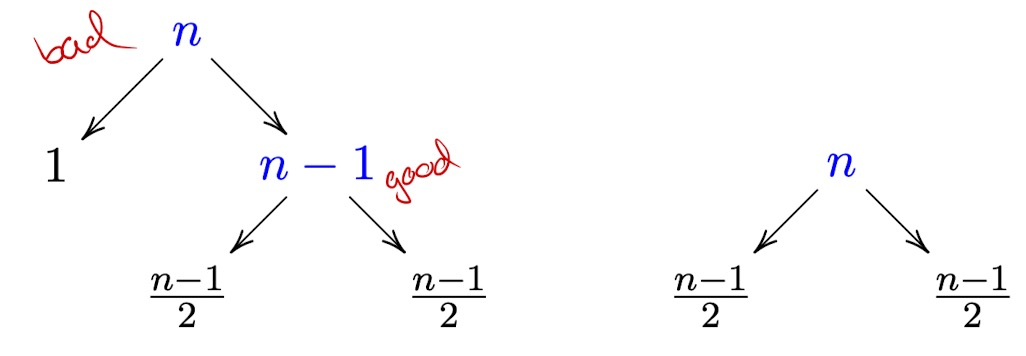
\includegraphics[width=0.5\linewidth]{images/Screenshot 2024-05-30 at 18.21.54.jpg}
    \end{figure}
    \item $G(n)=2B(n/2)+\Theta(n)$ and $B(n)=G(n-1)+\Theta(n)$
     \begin{align*}
        G(n)&=2B(n/2)+\Theta(n)\\
        &=2G(n/2-1)+\Theta(n/2)+\Theta(n)\\
        &=2G(n/2-1)+\Theta \leq 2G(n/2)+\Theta(n)
    \end{align*}
    \item It follows that, on average: $T(n)=\Theta(n \log_2 n)$
    \item Underlying assumption: all permutations of the input numbers are equally likely
    \item Randomized algorithm: partition around random item (instead of last item) 
\end{itemize}



\begin{minipage}{0.55\textwidth} % Adjust the width as needed
\centering % Center the content within the minipage
\begin{algorithm}[H]
\caption{RandomizedHoareParition(A,l,r)}
i = Random(l,r)\;
exchange A[i] and A[r]\;
\textbf{return} HoarePartition(A,l,r)\;
\end{algorithm}
\end{minipage}
\begin{minipage}{0.5\textwidth} % Adjust the width as needed
\centering % Center the content within the minipage
\begin{algorithm}[H]
\caption{RandomizedQuickSort(A,l,r)}
\If{$l<r$}{
m = RandomizedHoarePartition(A,l,r)\;
RandomizedQuickSort(A,l,m-1)\;
RandmoizedQuickSort(A,m,r)\;
}
\end{algorithm}
\end{minipage}
